\chapter{Technical Background}

This chapter will cover the following preliminary topics: cryptographic primitives, isogenies and their relevant properties, supersingular isogeny Diffie-Hellman (SIDH), the Fiat-Shamir construction for digital signatures (and its quantum-safe adaptation), current landscape of isogeny based signature schemes, and finally the C implementations of isogeny based schemes with which we are concerned.

In the first section of this chapter we will introduce a few cryptographic schemes for the readers who may not be entirely familiar with modern cryptography. We will cover key exchange, identification schemes, and signature schemes - all at as high of an abstraction level as possible. Readers familiar with these topics can skip this section without harm. 

Our discussion of isogenies will begin with some basic coverage of the underlying algebra. We will provide the material necessary for the remaining sections as we build up in the level of abstraction; working our way through groups, finite fields, elliptic curves, and finally isogenies and their properties.

Once we have presented the necessary algebra, we will illustrate the specifics of the supersingular isogeny Diffie-Hellman key-exchange protocol. We will spend most of this time dedicated to a modular deconstruction of the protocol, looking at the high-level procedures and algorithms which will be necessary for understanding in detail the signature protocol to come. This subsection will end with a briefing and analysis of the closely related zero-knowledge proof of identity (ZKPoI) isogeny protocol proposed in the original De Feo et al. paper\cite{djp}, as it is the foundation for the isogeny based signature scheme presented by Yoo et al\cite{yoo}.

In section 2.3 we will discuss the Fiat-Shamir transformation\cite{sigs}; a technique which, given a secure interactive proof of knowledge (\emph{identification scheme}), creates a secure digital signature scheme. We will also look at the quantum-secure adaptation published by Unruh\cite{unruh}, for applying a non-quantum-resistant transform to a quantum-resistant primitive would be rather frivolous.

Section 2.4 will be dedicated to covering current isogeny-based signature schemes - the topic of which this dissertation is mainly concerned. We will discuss the signature scheme of Yoo et al., which is a near direct application of Unruh's work to the SIDH zero-knowledge proof of identity.

Finally, the last section of this chapter will introduce the SIDH C library released by Microsoft Research, on top of which the core contributions of this thesis are implemented. We will also look at the implementation of the to-be-discussed signature scheme, which is a sort of proof-of-concept built ontop of the Microsoft API.\\


\section{Cryptographic Primitives}

Cryptographic primitives can be thought of as the basic building blocks used in the design of cryptographically secure applications. The idea of which being that if individual primitives are proven (or believeably) secure, we can be more confident in the security of the application as a whole.

To quickly recap some basic information security, there are serveral different security properties a cryptographic primitive may aim to offer:
\begin{itemize}
\item \emph{Confidentiality}:
The notion that the information in question is kept private from unauthorized individuals.
\item \emph{Integrity}:
The notion that the information in question has not been altered by unauthorized individuals.
\item \emph{Availability}:
The notion that the information in question is available to authorized individuals when requested.
\item \emph{Authenticity}:
The notion that the source of the information in question is verified.
\item \emph{Non-repudiation}:
The notion that the source of the information in question \textbf{cannot} deny having originally provided the information.
\end{itemize}

Each of the primitives to come are designed to offer some utility in the communication between a given pair of entities. We will refer to these entities as Alice and Bob. The schemes we are concerned with in this paper are strictly \emph{public key} (also known as \emph{asymmetric key}) schemes. In public key primitives, each user possesses a \emph{public} key (visible to every user in the network) as well as a \emph{private} key, which only they have access to. 

The first class of primitives we will discuss, \emph{key exchange} protocols, provide a means by which Alice and Bob can come to the agreement of some secret value. The goal of a key exchange protocol is for Alice \& Bob, communicating over some open, insecure channel, to reach mutual agreement of the secret value while also ensuring the \emph{confidentiality} of that value. The secret value is reffered to as a \emph{secret} or \emph{shared} key and is intended for use in other cryptographic primitives. 

Identification schemes are a class of primitives that aim to ensure \emph{authenticity} of a given entity. If Alice is communicating with Bob and she wants to verify that Bob is who he claims to be, the two can utilize a secure identification scheme. After identification protocols we will look at signature schemes, which are somewhat of an extension of the former. Signature schemes aim to provide \emph{authenticity} on every message sent from Bob to Alice, as well as \emph{non-repudiability} \& \emph{integrity} of those messages.\\

\subsection{Key Exchange}

A key exchange protocol, which we'll denote as $\Pi_{kex}$, can be represented in some contexts by a pair of polynomial time algorithms \textbf{KeyGen} and \textbf{SecAgr}: $\Pi_{kex} = (\textbf{KeyGen},\textbf{SecAgr})$. Alice and Bob will each run both of these procedures. The first they will run on the same input, $1^\lambda$, a bit string of $\lambda$ 1's. The second, short for ``secret agreement'', they will run on the output of $KeyGen$.\\

Execution of $\Pi_{kex}$ between Alice and Bob involves the following:
\begin{enumerate}[label=(\roman*)]
\item Alice and Bob run $\textbf{KeyGen}(1^\lambda)$: A probabilistic algorithm with input $1^\lambda$ and output $(sk,pk)$. Typically $pk$ is the image of $g(sk)$, where $h$ is some \emph{one-way} function.
\item Alice and Bob exchange (over an insecure channel) their public keys $pk_{\text{Alice}}$ and $pk_{\text{Bob}}$.
\item Alice runs $\textbf{SecAgr}(sk_{\text{Alice}}, pk_{\text{Bob}})$: A deterministic algorithm with input $sk_{\text{Alice}}$ and $pk_{\text{Bob}}$ and output $k_{\text{Alice}} \in \{0,1\}^\lambda$. Bob runs $\textbf{SecAgr}(sk_{\text{Bob}}, pk_{\text{Alice}})$.
\end{enumerate}

$\Pi_{kex}$ is said to uphold \emph{correctness} if $k_{Alice} = k_{Bob}$. Because we deal only with correct $\Pi_{kex}$, we refer to the output of $\Pi_{kex}$ as simply $k$. Figure \ref{fig:diffiehellman} illustrates an execution of the Diffie-Hellman key exchange protocol which relies on the difficulty of the \emph{discrete logarithm} problem for its one-way function $h$.\\

\begin{figure}[!h]
\begin{center}
\begin{tikzpicture}
  % Public parameter:
  \node[draw=none,fill=none,align=center] (public) at (0,1) {Public parameter:\\g, p};
  
  % Alice
  \node[draw] (Alice) at (-2,0) {Alice}; 
  \draw[thick] (Alice) -- ++(0, -4);
    
  % Calculations of Alice
  \node[draw=none,fill=none,anchor=east] (asecret) at ($(Alice) + (0,-1)$) {$a \in_{R} \{2,\dots,p-2\}$};
  \node[draw=none,fill=none,anchor=east] (Apublic) at ($(Alice) + (0,-2)$) {$A = g^{a} \bmod{p}$};
  \node[draw=none,fill=none,anchor=east] (akey) at ($(Alice) + (0,-4)$) {$K = (B)^{a} = g^{ba}$};
    
  % Bob
  \node[draw] (Bob) at (2,0) {Bob}; 
  \draw[thick] (Bob) -- ++(0, -4);
   
  % Calculations of Bob
  \node[draw=none,fill=none,anchor=west] (bsecret) at ($(Bob) + (0,-1)$) {$b \in_{R} \{2,\dots,p-2\}$};
  \node[draw=none,fill=none,anchor=west] (Bpublic) at ($(Bob) + (0,-2)$) {$B = g^{b} \bmod{p}$};
  \node[draw=none,fill=none,anchor=west] (bkey) at ($(Bob) + (0,-4)$) {$K = (A)^{b} = g^{ab}$};
   
  % Messages
  \draw[->,thick] ($(Alice)+(0,-2)$) -- ($(Bob)+(0,-2.5)$) node [pos=0.5,above,font=\footnotesize] {A};
  \draw[->,thick] ($(Bob)+(0,-3)$) -- ($(Alice)+(0,-3.5)$) node [pos=0.5,above,font=\footnotesize] {B};
    
\end{tikzpicture}
\end{center}
\caption{Alice and Bob's execution of Diffie-Hellman key exchange.}
\label{fig:diffiehellman}
\end{figure}

\subsection{Interactive Identification Schemes}

Imagine Alice wishes to confirm the identity of Bob. The idea behind interactive identification protocols is to offer Bob some way of proving to Alice (or anyone) that he has knowledge of some secret which \textbf{only} Bob could possess. The goal, of course, being to accomplish this without openly revealing the secret, so that it can continue to be used as an identifier for Bob. 

An identification scheme (or otherwise ``proof of knowledge" or ``proof of identity") $\Pi_{id}$ is composed of by the tuple of polynomial-time algorithms (\textbf{KeyGen}, \textbf{Prove}, \textbf{Verify}). $\Pi_{id}$ is an interactive protocol, wherein the \emph{prover} (Bob, for example) 
executes \textbf{Prove} and the \emph{verifier} (Alice) executes \textbf{Verify}.

Execution of $\Pi_{id}$ between Alice and Bob involves the following:
\begin{enumerate}[label=(\roman*)]
\item Bob runs $\textbf{KeyGen}(1^\lambda)$: A probabilistic algorithm with input $1^\lambda$ and output $(sk,pk)$. 
\item Bob sends to Alice his public key $pk$ and Alice will respond with a \emph{challenge} value $ch$.
\item Bob runs $\textbf{Prove}(sk, ch)$: A deterministic algorithm with input $sk$ (Bob's secret key) and $ch$ (challenge) and output $resp$.
\item Alice runs $\textbf{Verify}(pk, ch, resp)$: A deterministic algorithm with input $pk$ (Bob's public key), $ch$, and $resp$ and output $b \in {0,1}$. Bob has successfully proven his identity to Alice if $b = 1$.
\end{enumerate}

There exist variations upon this type of primitive wherein Alice is not required to send Bob a specific challenge value. These are known as \emph{non-interactive} identification schemes, or non-interactive proofs of identity (NIPoI). These non-interactive approaches to solving the problem of identity and \emph{authentication} further bridge the gap between identification protocols and signature schemes. 

\subsection{Signature Schemes}

There are two main differences between signature schemes and interactive identification schemes. The first is equivalent to the difference between Second, because we wish to authenticate Bob on every message, our scheme needs to be run every time Bob wishes to send a message to Alice. We must also include Bob's message $m$ in our execution of \textbf{Verify} (which in the context of signatures, we call \textbf{Sign}). And so, a signature scheme can be thought of as an NIPoI executed with respect to a particular message. We define a signature scheme as the tuple of algorithms $\Pi_{sig}$ = (\textbf{KeyGen}, \textbf{Sign}, \textbf{Verify}).

Execution of $\Pi_{sig}$ between Alice and Bob for a particular message $m$ sent from Bob to Alice involves the following:
\begin{enumerate}[label=(\roman*)]
\item Bob runs $\textbf{KeyGen}(1^\lambda)$: A probabilistic algorithm with input $1^\lambda$ and output $(sk,pk)$.
\item Bob sends his public key to Alice.
\item Bob runs $\textbf{Sign}(sk, m)$: A deterministic algorithm with input $sk$ (Bob's secret key) and $m$ (the message Bob wishes to authorize) and output $\sigma$, known as a \emph{signature}.
\item Bob sends $m$ and $\sigma$ to Alice.
\item Alice runs $\textbf{Verify}(pk, m, \sigma)$: A deterministic algorithm with input $pk$ (Bob's public key), $m$, and $\sigma$ and output $b \in {0,1}$. Alice has confidence in the \emph{integrity} and origin \emph{authenticity} of $m$ if $b = 1$.
\end{enumerate}

\section{Algebraic Geometry \& Isogenies}
\emph{Groups \& Varieties}. A \textbf{group} is a 2-tuple composed of a set of elements and a corresponding group operation (also referred to as the group \emph{law}). Given some group defined by the set $G$ and the operation $\cdot$ (written as $(G,\cdot)$) it is typical to refer to the group simply as $G$. If $\cdot$ is equivalent to some rational mapping[footnote about rational mappings] $f_G: G \rightarrow G$, then the group $(G,\cdot)$ is said to form an \textit{algebraic variety}[footnote about the inverse function]. A group which is also an algebraic variety is referred to as an \textbf{algebraic group}.

$G$ is said to be an \emph{abelian} group if, in addition to the four traditional group axioms (closure, associativity, existence of an identity, existence of an inverse), $G$ satisfies the condition of commutitiviy. More formally, for some group $G$ with group operation $\cdot$, we say $G$ is an abelian group iff $x \cdot y = y \cdot x$ $\forall x, y \in G$. An algebraic group which is also abelian is referred to as an \textbf{abelian variety}.

\begin{tcolorbox}
\begin{definition}[Abelian Variety]
\label{defn:abelianvariety}
for some algebraic group $G$ with operation $\cdot$, we say $G$ is an \underline{abelian variety} iff $x \cdot y = y \cdot x$ $\forall x, y \in G$. 
\end{definition}
\end{tcolorbox}

For some group $(G,\cdot)$, some $x,y \in G$, and some rational mapping $f_G: G \rightarrow G$, let the following sequence of implications denote the classification of $(G,\cdot)$:

$$
\text{group } \xRightarrow[]{x\cdot y = f_G(x,y)} \text{algebraic group } \xRightarrow[]{x\cdot y = y\cdot x} \text{abelian variety }
$$


\noindent
\emph{Morphisms}. Let us again take for example some group $(G,\cdot)$. Let's also define some set $S_{(G,\cdot)}$ which contains every tuple $(x,y,z)$ for group elements $x,y,z$ which satisfy $x\cdot y = z$.
$$
S_{(G,\cdot)} = \{x,y,z \in G | x\cdot y = z\}
$$
Take also for example a second group $(H,*)$ and some map $\phi: G \rightarrow H$. $\phi$ is said to be \emph{structure preserving} if the following implication holds:
$$
(x,y,z) \in S_{(G,\cdot)} \Rightarrow (\phi(x),\phi(y),\phi(z)) \in S_{(H,*)}
$$

A \textbf{morphism} is simply the most general notion of a structure preserving map. More specifically, in the domain of algebraic geometry, we will be dealing with the notion of a \textbf{group homomorphism}, defined as follows:
\begin{tcolorbox}
\begin{definition}[Group Homomorphism]
\label{defn:homomorphism}
For two groups $G$ and $H$ with respective group operations $\cdot$ and $*$, a \underline{group homomorphism} is a structure preserving map $h: G \rightarrow H$ such that $\forall u, v \in G$ the following holds:
$$h(u \cdot v) = h(u) * h(v)$$
\end{definition}
\end{tcolorbox}

From this simple definition, two more properties of homomorphisms are easily deducible. Namely, for some homomorphism $h: G \rightarrow H$, the following properties hold:
\begin{itemize}
\item $h$ maps the identity element of $G$ onto the identity element of $H$, and
\item $h(u^{-1}) = h(u)^{-1}, \forall u \in G$
\end{itemize}

Furthermore, an \emph{endomorphism} is a special type of morphism in which the domain and the codomain are the same groups. We denote the set of enomorphisms defineable over some group $G$ as $\text{End}(G)$.
The \emph{kernel} of a particular homomorphism $h: G \rightarrow H$  is the set of elements in $G$ that, when applied to $h$, map to the identity element of $H$. We write this set as $ker(h)$, and it is much analogous to the familiar concept from linear algebra, wherein the kernel denotes the set of elements mapped to the zero vector by some linear map.
\vspace{10mm}

\noindent
\emph{Fields \& Field Extensions}. A \textbf{field} is a mathematical structure which, while being similar to a group, demands additional properties. Fields are defined by some set $F$ and two operations: \emph{addition} and \emph{multiplication}. In order for some tuple $(F,+,\cdot)$ to constitute a field, it must satisfy an assortment of axioms:\\

\emph{addition axioms}:
\begin{itemize}
\item If $x \in F$ and $y \in F$, then $x + y \in F$.
\item $+$ is commutative.
\item $+$ is associative.
\item $F$ contains an element 0 such that $\forall x \in F$ we have $0 + x = x$.
\item $\forall x \in F$ there is a corresponding element $-x \in F$ such that $x + (-x) = 0$.
\end{itemize}

\emph{multiplication axioms}:
\begin{itemize}
\item If $x \in F$ and $y \in F$, then $x \cdot y \in F$.
\item $\cdot$ is commutative.
\item $\cdot$ is associative.
\item $F$ contains an element $1 \neq 0$ such that $\forall x \in F$ we have $x \cdot 1 = x$.
\item $\forall x \neq 0 \in F$ there is a corresponding element $1/x \in F$ such that $x \cdot (1/x) = 1$.
\end{itemize}

Additionally, a field $(F,+,\cdot)$ must uphold the \emph{distributive law}, namely:
$$
 x \cdot (y + z) = x \cdot y + x \cdot y \text{ holds } \forall x,y,z \in F
$$

While these axioms are known to be satisfied by the sets $\mathbb{Q}$, $\mathbb{R}$, and $\mathbb{C}$ with typically defined $+$ and $\cdot$, our focus will be on a particular class of field known as a \emph{finite field}. Finite fields, as the name suggests, are fields in which the set $F$ contains finitely many elements - we refer to the number of elements in $F$ as the \emph{order} of the field.

Let us take some prime number $p$. We can construct a finite field by taking $F$ as the set of numbers $\{0, 1, ... p-1\}$ and defining $+$ and $\cdot$ as addition and multiplication \emph{modulo p}. Finite fields defined in this fashion are denoted as $\mathbb{F}_p$, and have order $p$.
\begin{center}
$\forall x,y \in \mathbb{F}_p$, $x + y = (x + b) \mod{p}$, and\\
$\forall x,y \in \mathbb{F}_p$, $x \cdot y = (x \cdot b) \mod{p}$\\
\end{center}

For any given field $K$ there exists a number $q$ such that, for every $x \in K$, adding $x$ to itself $q$ times results in the additive identity 0. This number is referred to as the \emph{characteristic} of $K$, for which we write char($K$). Finite fields are the only type of field for which $\text{char}(K) > 0$. Furthermore, if the field in question is finite and has prime order, then the order and the characteristic are equivalent.

A particular field $K'$ is called an \emph{extension field} of some other field $K$ if $K \subseteq K'$. The complex numbers $\mathbb{C}$, for example, are an extension field of $\mathbb{R}$. A given field $K$ is \emph{algebraically closed} if there exists a root for every non-constant polynomial defined over $K$. If $K$ itself is not algebraically closed, we denote the extension of $K$ that is by $\overline{K}$. 

An algebraic group $G_a$ is defined over a field $K$ if each element $e \in G_a$ is defined over $K$ and the corresponding $f_{G_a}$ is also defined over $K$. To show that a particular algebraic group $G_a$ is defined over some field $K$ we will henceforth denote the group/field pairing as $G_a(K)$. Naturally, in the case where our field is a finite field of order $p$, we write $G_a(\mathbb{F}_p)$.

These algebraic structures are all important for building up to the concept of an \emph{isogeny}. The lowest-level object we will be concerned with when discussing the forthcoming isogeny-based protocols will typically be elements of abelian varieties. The lowest-level structure in the SIDH C codebase is a finite field element.\\

\subsection{Elliptic Curves}

An elliptic curve is an algebraic curve defined over some field $K$, the most general representation of which is given by
$$
y^2 + a_{1}xy + a_{3}y = x^3 + a_{2}x^2 + a_{4}x + a_6.
$$
This representation encapsulates elliptic curves defined over any field. If, however, we are dicussing curves defined specifically over a field $K$ such that $\text{char}(K) > 3$[ref], then the more compact form $y^2 = x^3 + ax + b$ can be applied (see figure \ref{fig:groupop} for a geometric visualization). In this dissertation we will default to this second representation, as the schemes with which we are concerned will always be defined over $\mathbb{F}_p$ for some large prime $p$.

Within algebraic geometry, it is common practice to define a group structure over the points of a given elliptic curve (or any other smooth cubic curve). If we wish to define a group in accordance to a particular curve, we do so with the following notation:
$$
E: y^2 = x^3 + ax + b
$$
Wherein $E$ denotes the group in question, the elements of which are all the points (solutions) of the curve. Throughout much of this section, the words \emph{point} and \emph{element} can be used interchangeably.\\

\noindent
\emph{The Group Law}. The group operation we define for $E$, denoted $+$, is better understood geometrically than algebraically. Consider the following.

Given two elements $P$ and $Q$ of some arbitrary elliptic curve group $E$, we define $+$ geometrically as follows: drawing the line $L$ formed by points $P$ and $Q$, we follow $L$ to its third intersection on the curve, which we will denote as $R = (x_R, y_R)$. We then set $P + Q = -R$, where $-R$ is the reflection of $R$ over the x-axis: $(x_R, -y_R)$. See figure \ref{fig:groupop} for an illustrated representation of this process.

\begin{figure}[!h]
\begin{tikzpicture}[scale=.75]
	\begin{scope}[xshift=5cm]
		%\draw[very thin,color=gray] (-3.9,-3.9) grid (3.9,3.9);  %background grid
		\draw[->] (-4.2,0) -- (4.2,0) node[right] {$x$};         %x-axis
		\draw[->] (0,-4.2) -- (0,4.2) node[above] {$y$};         %y-axis
		
		\plotcurve{-2}{2}
		
		\draw[fill] (-1.73,0.531) circle (0.1) node[right] {$P$};
		\draw[fill] (0.28,1.209) circle (0.1) node[right] {$Q$};
	\end{scope}
	
	\begin{scope}[xshift=17cm]
		%\draw[very thin,color=gray] (-3.9,-3.9) grid (3.9,3.9);  %background grid
		\draw[->] (-4.2,0) -- (4.2,0) node[right] {$x$};         %x-axis
		\draw[->] (0,-4.2) -- (0,4.2) node[above] {$y$};         %y-axis
		
		\plotcurve{-2}{2}
		
		\draw [] (-1.73,0.531) -- (1.564,1.642);
		\draw [dashed] (1.564,1.642) -- (1.564,-1.642);
		
		\draw[fill] (-1.73,0.531) circle (0.1) node[right] {$P$};
		\draw[fill] (0.28,1.209) circle (0.1) node[right] {$Q$};
		\draw[fill] (1.564,1.642) circle (0.1) node[right] {$R$};
		\draw[fill] (1.564,-1.642) circle (0.1) node[right] {$R' = P+Q$};
  \end{scope}
\end{tikzpicture}
\caption{$+$ acting over points $P$ and $Q$ of $y^2 = x^3 - 2x + 2$.}
\label{fig:groupop}
\end{figure}

The group operation $+$ is referred to as \emph{pointwise addition}. In order for $(E,+)$ to properly form a group under pointwise addition, it must satisfy the four group axioms:
\begin{itemize}
\item \emph{Closure}: Because elliptics curves are polynomials of degree of 3, we know any given line passing through two points $P$ and $Q$ of $E$ will pass through a third point $R$. The exceptions here are twofold. First, when $P = Q$ and thus our line is tangent to $E$, and second, when $Q = -P$ and our line is parallel with the y-axis. We resolve the first case nicely by defining $P + P$ by means of taking $L$ to be the line tangent to $E$ at point $P$. In the second case, $P + (-P)$, by group axiom, should yield the identity element of the group. We will define this element and resolve this issue below.  
\item \emph{Identity}: The identity element of elliptic curve groups, denoted as $\mathcal{O}$, is a specially defined point satisfying $P + \mathcal{O} = \mathcal{O} + P = P$, $\forall P \in E$. Because of the inclusion of this special element, we have that $\#(E(K))$ is equal to $1$ $+$ the number geometric points on $E$ defined over $K$. This of course is only a noteworthy claim when $K$ is a finite field (otherwise there are already infinitely many elements in $E$).
\item \emph{Associativity}: To show that associativity holds for geometrically defined points $P$, $Q$, and $R$ in $E$ ($(P + Q) + R = P + (Q + R)$) is rather simple (see figure \ref{fig:axioms}). We can trivially show that this holds when any combination of $P$, $Q$, and $R$ are $\mathcal{O}$ by applying the axiom of the identity.
\item \emph{Inverse}: Due to the x-symmetry of elliptic curves, every point $P = (x_P, y_P)$ of $E$ has an associated point $-P = (x_P, -y_P)$. If we apply $+$ to $P$ and $-P$, $L$ assumes the line parrallel to the y-axis at $x = x_P$. As discussed above, in this case there is no third intersection of $L$ on $E$. In light of this, $\mathcal{O}$ can be thought of as a point residing infinitely far in both the positive and negative directions of the y-axis. $\mathcal{O}$ is equivalently referred to as the \emph{point at infinity}.[footnote about whether $+$ actually constitutes a rational map due to this exception]
\end{itemize}

\begin{figure}[!h]
\begin{tikzpicture}[scale=.55]
	\begin{scope}[xshift=0cm]
		%\draw[very thin,color=gray] (-3.9,-3.9) grid (3.9,3.9);  %background grid
		\draw[->] (-4.2,0) -- (4.2,0) node[right] {$x$};         %x-axis
		\draw[->] (0,-4.2) -- (0,4.2) node[above] {$y$};         %y-axis
		
		\draw[] (-1.65,0.677) -- (2.00,1.414); 
		\draw[dashed] (-0.309,0.948) -- (-0.309,-0.948);
		\draw[] (-1.400,-1.207) -- (1.765,-0.454); 
		\draw[dashed] (1.765,-0.454) -- (1.765,0.454);
		
		\plotcurve{-3}{0}
		
		\draw[fill] (-1.65,0.677) circle (0.1) node[left] {$P$};
		\draw[fill] (2.00,1.414) circle (0.1) node[right] {$Q$};
		\draw[fill] (-0.309,0.948) circle (0.1) node[right] {};
		\draw[fill] (-0.309,-0.948) circle (0.1) node[right] {};
		\draw[fill] (-1.400,-1.207) circle (0.1) node[below] {$R$};
		\draw[fill] (1.765,-0.454) circle (0.1) node[right] {};
		\draw[fill] (1.765,0.454) circle (0.1) node[right] {$(P + Q) + R$};
	\end{scope}
	\begin{scope}[xshift=10cm]
		%\draw[very thin,color=gray] (-3.9,-3.9) grid (3.9,3.9);  %background grid
		\draw[->] (-4.2,0) -- (4.2,0) node[right] {$x$};         %x-axis
		\draw[->] (0,-4.2) -- (0,4.2) node[above] {$y$};         %y-axis
		
		\draw[] (2.00,1.414) -- (-1.400,-1.207);
		\draw[dashed] (-0.006,-0.132) -- (-0.006,0.132);
		\draw[] (-1.65,0.677) -- (1.765,-0.454);
		\draw[dashed] (1.765,-0.454) -- (1.765,0.454);
		
		\plotcurve{-3}{0}
		
		\draw[fill] (-1.65,0.677) circle (0.1) node[left] {$P$};
		\draw[fill] (2.00,1.414) circle (0.1) node[right] {$Q$};
		\draw[fill] (-1.400,-1.207) circle (0.1) node[below] {$R$};
		\draw[fill] (-0.006,-0.132) circle (0.1) node[right] {};
		\draw[fill] (-0.006,0.132) circle (0.1) node[right] {};
		\draw[fill] (1.765,-0.454) circle (0.1) node[right] {};
		\draw[fill] (1.765,0.454) circle (0.1) node[right] {$P + (Q + R)$};
	\end{scope}
	\begin{scope}[xshift=20cm]
		%\draw[very thin,color=gray] (-3.9,-3.9) grid (3.9,3.9);  %background grid
		\draw[->] (-4.2,0) -- (4.2,0) node[right] {$x$};         %x-axis
		\draw[->] (0,-4.2) -- (0,4.2) node[above] {$y$};         %y-axis
		
		\plotcurve{1}{1}
		
		\draw[dashed] (0.73,-4.492) -- (0.73,4.492);
		
		\draw[fill] (0.73,1.492) circle (0.1) node[right] {$P$};
		\draw[fill] (0.73,-1.492) circle (0.1) node[right] {$-P$};
  \end{scope}
\end{tikzpicture}
\caption{associativity illustrated on $y^2 = x^3 - 3x$ (left \& center) and $P + (-P) = \mathcal{O}$ illustrated for $y^2 = x^3 + x + 1$ (right).}
\label{fig:axioms}
\end{figure}

Additionally, we shorthand $\overbrace{P + P + ... + P}^{n}$ as $nP$, analogous to scalar multiplication.\\

Consequently, because groups defined over elliptic curves in this fashion are commutitive, they also constitute abelian varieties[ref].

When referring to curves as abelian varieties defined over a field, we will write them as $E_{\alpha}(K)$, for some curve $E_{\alpha}$ and some field $K$. If we are only concerned with the geometric properties of the curve, or curves as distinct elements of some group structure, it will suffice to write $E_{\alpha}$. Moving forward from here, we will assume all general curves discussed are capable of definition over some finite field $\mathbb{F}_p$.\\

\noindent
\emph{Torsion Groups}. The $r$-\emph{torsion group} of $E$ is the set of all points $P \in E(\overline{\mathbb{F}}_q)$ such that $[r]P = \mathcal{O}$. We denote the $r$-torsion group of some curve as $E[r]$.\\

\noindent
\emph{Supersingular Curves}. An elliptic curve can be either \emph{ordinary} or \emph{supersingular}. There are several equivalent ways to define supersingular curves (and thus the distinction between them and ordinary curves,)

For the remainder of this paper, unless otherwise noted, all elliptic curves in discussion will be of the supersingular variety.\\

\noindent
\emph{Montgomery Arithmetic}.

\subsection{Isogenies \& Their Properties}

\begin{tcolorbox}
\begin{definition}[Isogeny]
\label{defn:isogeny}
Let $G$ and $H$ be algebraic groups[ref]. An \underline{isogeny} is a morphism[ref] $h: G \rightarrow H$ possessing a finite kernel.
\end{definition}
\end{tcolorbox}

In the case of the above definition where $G$ and $H$ are abelian varieties (such as elliptic curves,) the isogeny $h$ is homomorphic[ref] between $G$ and $H$. Because of this, isogenies over elliptic curves (and other abelian varieties) inherit certain characteristics.\\
For an isogeny $h: E_{1} \rightarrow E_{2}$ defined over elliptic curves $E_1$ and $E_2$, the following holds:
\begin{itemize}
\item $h(\mathcal{O}) = \mathcal{O}$, and
\item $h(u^{-1}) = h(u)^{-1}, \forall u \in G$
\end{itemize}

We write $\text{End}(E)$ to denote the ring formed by all the isogenies acting over $E$ which are also endomorphisms. Note that $m$-repeated pointwise addition of a point with itself can equivalently be modelled by an endomorphism, we denote the application of such an endomorphism to a point $P$ as $[m]P$, such that $[m]: E \rightarrow E$ and $[m]P = mP$.

\section{Supersingular Isogeny Diffie-Hellman}

This section will aim to accomplish two things. First, we will briefly explain the isogeny-level \& key-exchange-level procedures of the SIDH protocol. Second, we will illuminate how these procedures map onto Microsoft Research's C implementation of SIDH. In this regard, this section can be considered an attempt to meld two domains of SIDH functions \& procedures, in hopes of easing the navigation from the SIDH protocol to Microsoft's C implementation, and vice versa.

The original work of De Feo, Jao, and Plut outlines three different isogeny-based cryptographic primitives: Diffie-Hellman-esque key exchange, public key encryption, and the aforementioned zero-knowledge proof of identity. Because all three of these protocols require the same initialization and public parameters, we will begin by covering these parameters in detail. Immediately after, we will analyze the key exchange at a relatively high level. Our goal of this section is to explain in detail the algorithmic and cryptographic aspects of the ZKPoI scheme, as this forms the conceptual basis for the signature scheme we will be investigating. We begin with the key exchange protocol because its sub-routines are integral to the Yoo et al. signature implementation.

For the discussion that follows, we will assume every instance of an SIDH protocol occurs between two parties, \textcolor{blue}{A} and \textcolor{red}{B} (eg. \textcolor{blue}{Alice} \& \textcolor{red}{Bob},) for which we will colorize information particular to \textcolor{blue}{A} in \textcolor{blue}{blue} and \textcolor{red}{B} in \textcolor{red}{red}. This will include private keys \& public keys as well as the variables and constants used in their generation.

\subsection{Public Parameters}

As the name suggests, SIDH protocols work over supersingular curves (with no singular points). Let $\mathbb{F}_q = \mathbb{F}_{p^2}$ be the finite field over which our curves are defined, $\mathbb{F}_{p^2}$ denoting the quadratic extension field of $\mathbb{F}_{p}$.  $p$ is a prime defined as follows:
$$
p = \laea \lbeb \cdot f \pm 1
$$
Wherein $\la$ and $\lb$ are small primes (typically \textcolor{blue}{2} \& \textcolor{red}{3}, respectively) and $f$ is a cofactor ensuring the primality of $p$. We then define globally a supersingular curve $E_0$ defined over $\mathbb{F}_q$ with cardinality $(\laea \lbeb f)^2$. Consequently, the torsion group $E_0[\laea]$ is $\mathbb{F}_q$-rational and has $\la^{\ea - 1} (\la + 1)$ cyclic subgroups of order $\laea$, with the analogous statement being true for $E_0[\lbeb]$. Additionally, we include in the public parameters the bases $\agens$ and $\bgens$, generating $E[\laea]$ and $E[\lbeb]$ respectively. 

This brings our set of global parameters, G, to the following:\\
$$
G = \{p,E_0,\la,\lb,\ea,\eb,\agens,\bgens\}
$$



\subsection{SIDH Key Exchange}

This subsection will illustrate an SIDH key exchange run between party members \textcolor{blue}{Alice} and \textcolor{red}{Bob}. The general idea of the protocol can be surmised by the diagram below. In the scheme, \textbf{private keys} take the form of isogenies[ref] defined with domain $E$, and \textbf{public keys} are the associated co-domain curve of said isogenies.

\begin{center}
\begin{tikzpicture}
  \matrix (m) [matrix of math nodes,
               row sep=4em,
               column sep=4em,
               minimum width=2em] {
    E_0                     & E_0 / \langle \textcolor{blue}{A} \rangle    \\
    E_0 / \langle \textcolor{red}{B} \rangle & E_0 / \langle \textcolor{blue}{A}, \textcolor{red}{B} \rangle \\
  };
  \path[-stealth]
    (m-1-1) edge node [above] {$\pa$}  (m-1-2)
    (m-1-1) edge node [left]  {$\pb$}  (m-2-1)
    (m-2-1) edge node [below] {$\pap$} (m-2-2)
    (m-1-2) edge node [right] {$\pbp$} (m-2-2);
\end{tikzpicture}
\end{center}

The premise of the protocol is that both parties generate some random point (\textcolor{blue}{A} or \textcolor{red}{B} in the diagram,) which, according to theorem [ref], indicates some distinct isogeny $\phi_{\ba}: E_0 \rightarrow E/ \langle \ba \rangle$ (or equivalent for \rb). \textcolor{blue}{Alice} and \textcolor{red}{Bob} then exchange codomain curves and compute
\begin{center}
$\pa(E_0/\langle \rb \rangle)$\\
$\text{OR}$\\
$\pb(E_0/\langle \ba \rangle)$
\end{center}
To come to the shared secret agreement, the codomain curve of their composed isogenies, denoted $E_{\ba\rb}$. Below we've outlined the SIDH key exchange protocol $\Pi_{\text{SIDH}}$ = (\textbf{KeyGen}, \textbf{SecAgr}) in a descriptive (though not yet algorithmic) manner.\\

\noindent
\textbf{KeyGen}: \textcolor{blue}{Alice} chooses two random numbers $\ma, \na \in \mathbb{Z}/\laea\mathbb{Z}$ such that $(\la \nmid \ma) \lor (\la \nmid \na)$. \textcolor{blue}{Alice} then computes the isogeny $\pa: E_0 \rightarrow E_{\ba}$ where $E_{\ba} = E_0 / \langle [\ma]\genpa, [\na]\genqa\rangle$ (equivalently, $ker(\pa) = \langle [\ma]\genpa, [\na]\genqa\rangle$). \bob undergoes the same procedure for random elements $\mb, \nb \in \mathbb{Z}/\lbeb\mathbb{Z}$. After completion, \alice and \bob hold their respective key pairs:
\begin{center}
$(sk_A, pk_A) = (\{\ma,\na\}, E_{\ba})$\\
$(sk_B, pk_B) = (\{\mb,\nb\}, E_{\rb})$\\
\end{center}

\alice then applies her isogeny to the points which \bob will use in the creation of of his isogeny: $\{\pa(\genqb),\pa(\genqb)\}$. \bob performs the analogous operation.\\

\noindent
\textit{PK Exchange}: After \textcolor{blue}{Alice} and \textcolor{red}{Bob} successfully complete their key generation, they perform the following over an insecure channel:\\
\begin{itemize}
\item \alice sends \bob $(E_{\ba}, \{\pa(\genpb),\pa(\genqb)\})$
\item \bob sends \alice $(E_{\rb}, \{\pb(\genpa),\pb(\genqa)\})$
\end{itemize}

\noindent
\textbf{SecAgr}: After reception of \bob's tuple, \alice computes the isogeny $\phi'_A: E_{\rb} \rightarrow E_{\ba\rb}$ and \bob acts analogously. \alice and \bob then arrive at the equivalent image curve:
$$
E_{\ba\rb} = \phi'_{\ba}(\phi_{\rb}(E_0)) = \phi'_{\rb}(\phi_{\ba}(E_0)) = E_0/ \langle [\ma]\genpa + [\na]\genqa, [\mb]\genpb + [\nm]\genqb \rangle
$$
From which they can use the common j-invariant of as a shared secret $k$.

\begin{figure}[htb]
\centering
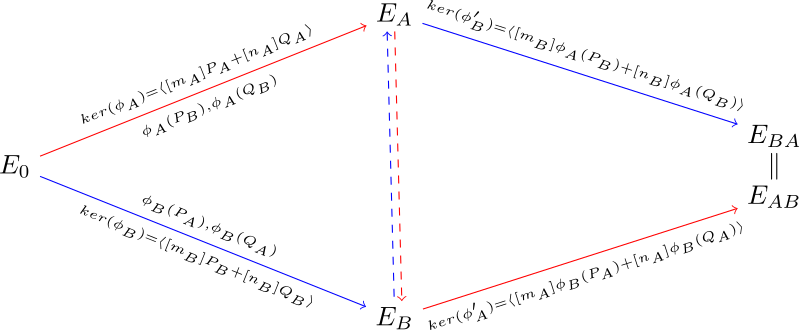
\includegraphics[scale=0.5]{keyexchange.png} % e.g. insert ./image for image.png in the working directory, adjust scale as necessary
\caption{SIDH key exchange between \textcolor{blue}{Alice} \& \textcolor{red}{Bob}}
\label{fig:kex} % insert suitable label, this is used to refer to a fig from within the text as shown above
\end{figure}

\subsection{Zero-Knowledge Proof of Identity}

Recall the notion of a simple identification scheme:

\section{Fiat-Shamir Construction}

The Fiat-Shamir construction (sometimes referred to as the Fiat-Shamir heuristic or transform) is used

\subsection{Unruh's Post-Quantum Adaptation}


\section{Isogeny Based Signatures}

Now that we've introduced the zero-knowledge proof of identity scheme from [REFERENCE] as well as Unruh's quantum-safe Fiat-Shamir adaption, the isogeny based signature scheme presented by Yoo et. Al is a near-trivial application of the latter to the former. 

The isogeny based signature scheme presented by Yoo et. Al is defined, in the traditional manner, by a tuple of algorithms. Namely, the scheme is defined by the tuple (KeyGen, Sign, Verify) with each algorithm loosely defined as follows:\\
\textbf{KeyGen(}\textbf{)}: Select a random point $S$ of order $\ell_{A}^{e_A}$, compute the isogeny $\phi: E \rightarrow E/ \langle S \rangle$. Return (pk, sk) where pk = $(E/ \langle S \rangle, \phi(P_B), \phi(Q_B))$ and sk = $S$.\\
\textbf{Sign()}:\\
\textbf{Verify()}:\\


\section{Implementations of Isogeny Based Schemes}

\subsection{Parameters}

Figure [ref] illustrates the relationship between abstraction levels of the SIDH protocol and modules of the SIDH C library.\\

\noindent
\emph{Key Representation}.

\begin{figure}[htb]
\centering
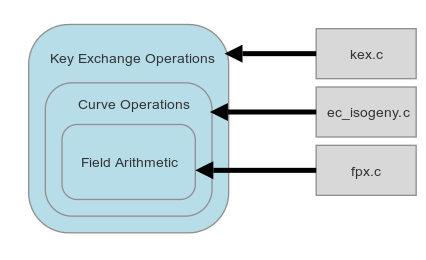
\includegraphics[scale=0.7]{halfmapwcurve.png} % e.g. insert ./image for image.png in the working directory, adjust scale as necessary
\caption{Relationship between SIDH key exchange \& MR SIDH C library}
\label{fig:halfmap} % insert suitable label, this is used to refer to a fig from within the text as shown above
\end{figure}

\subsection{Yoo et al. Signature Layer}

\begin{figure}[htb]
\centering
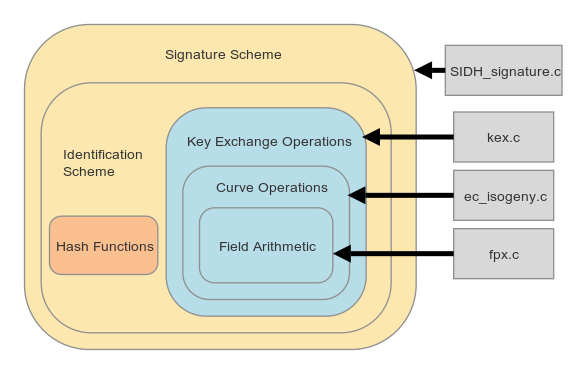
\includegraphics[scale=0.7]{fullmapwcurve.png} % e.g. insert ./image for image.png in the working directory, adjust scale as necessary
\caption{Relationship between SIDH based signatures \& Our fork of the SIDH C library}
\label{fig:fullmap} % insert suitable label, this is used to refer to a fig from within the text as shown above
\end{figure}


Shortly after, the following, more in-depth algorithms are given as definitions: 

\begin{algorithm}
\caption{KeyGen($\lambda$)}\label{euclid}
\begin{algorithmic}[1]
\State Pick a random point S of order $\ell^{e_{A}}_{A}$
\State Compute the isogeny $\phi: E \rightarrow E/\langle S \rangle$
\State pk $\gets (E/\langle S \rangle, \phi(P_{B}), \phi(Q_{B}))$
\State sk $\gets S$
\State \Return (pk,sk)
\end{algorithmic}
\end{algorithm}

\begin{algorithm}
\caption{Sign(sk, $m$)}\label{euclid}
\begin{algorithmic}[1]
\For{\texttt{i = 1..2$\lambda$}}
	\State Pick a random point R of order $\ell^{e_{B}}_{B}$
	\State Compute the isogeny $\psi: E \rightarrow E/\langle R \rangle$
	\State Compute either $\phi' : E/\langle R \rangle \rightarrow E/\langle R,S \rangle$ or $\psi' : E/\langle S \rangle \rightarrow E/\langle R,S \rangle$
	\State $(E_{1},E_{2}) \gets (E/\langle R \rangle, E/\langle R,S \rangle)$
	\State $\texttt{com}_{i} \gets (E_{1}, E_{2})$
	\State $\texttt{ch}_{i,0} \gets_{R} \{0,1\}$
	\State $(\texttt{resp}_{i,0}, \texttt{resp}_{i,1}) \gets ((R,\phi(R)), \psi(S))$
	\If{$\texttt{ch}_{i,0} = 1$}
		\State $\texttt{swap}(\texttt{resp}_{i,0},\texttt{resp}_{i,1})$
	\EndIf
	\State $h_{i,j} \gets G(\texttt{resp}_{i,j})$
\EndFor

\State $J_{1} \parallel ... \parallel J_{2\lambda} \gets H(pk, m, (\texttt{com}_{i})_{i},(\texttt{ch}_{i,j})_{i,j},(h_{i,j})_{i,j})$

\State \Return $\sigma \gets ((\texttt{com}_{i})_{i}, (\texttt{ch}_{i,j})_{i,j}, (h_{i,j})_{i,j}, (\texttt{resp}_{i,J_{i}})_{i})$
\end{algorithmic}
\end{algorithm}

\begin{algorithm}[H]
\caption{Verify(pk, $m$, $\sigma$)}\label{euclid}
\begin{algorithmic}[1]
\State $J_{1} \parallel ... \parallel J_{2\lambda} \gets H(pk, m, (\texttt{com}_{i})_{i},(\texttt{ch}_{i,j})_{i,j},(h_{i,j})_{i,j})$
\For{\texttt{i = 0..2$\lambda$}}
	\State \textbf{check} $h_{i,J_{i}} = G(\texttt{resp}_{i,J_{i}})$
	\If{$\texttt{ch}_{i,J_{i}} = 0$}
		\State Parse $(R,\phi(R)) \gets \texttt{resp}_{i,J_{i}}$
		\State \textbf{check} $(R, \phi(R))$ have order $\ell^{e_{B}}_{B}$
		\State \textbf{check} $R$ generates the kernel of the isogeny $E \rightarrow E_{1}$
		\State \textbf{check} $\phi(R)$ generates the kernel of the isogeny $E/\langle S \rangle \rightarrow E_{2}$
	\Else
		\State Parse $\psi(S) \gets \texttt{resp}_{i,J_{i}}$
		\State \textbf{check} $\psi(S)$ has order $\ell^{e_{A}}_{A}$
		\State \textbf{check} $\psi(S)$ generates the kernel of the isogeny $E_{1} \rightarrow E_{2}$
	\EndIf
\EndFor

\If{all checks succeed}
	\State \Return 1
\EndIf
\end{algorithmic}
\end{algorithm}

If we transcribe the above to the language of the Microsoft SIDH API, we have in essense the following:\\

\begin{algorithm}
\caption{KeyGen($\lambda$)}\label{euclid}
\begin{algorithmic}[1]
\State (pk, sk) $\gets \texttt{KeyGeneration\_B()}$
\State \Return (pk,sk)
\end{algorithmic}
\end{algorithm}

\begin{algorithm}
\caption{Sign(sk, $m$)}\label{euclid}
\begin{algorithmic}[1]
\For{\texttt{i = 1..2$\lambda$}}
	\State $(, R, \psi) \gets \texttt{KeyGeneration\_A(E)}$
	\State $E_{1} \gets E/\langle R \rangle$
	\State $(E_{2},E/\langle R,S \rangle) \gets \texttt{SecretAgreement\_B()}$
	\State $(E_{1},E_{2}) \gets (E/\langle R \rangle, E/\langle R,S \rangle)$
	\State $\texttt{com}[i] \gets (E_{1}, E_{2})$
	\State $\texttt{ch}[i] \gets_{R} \{0,1\}$
	\State $(\texttt{resp}[i]_{0}, \texttt{resp}[i]_{1}) \gets ((R,\phi(R)), \psi(S))$
	
%% this portion was skipped?	
%%	\If{$\texttt{ch}[i] = 1$}
%%		\State $\texttt{swap}(\texttt{resp}[i]_{0},\texttt{resp}[i]_{1})$
%%	\EndIf
%%	\State $h_{i,j} \gets G(\texttt{resp}[i]_{j})$
\EndFor

\State $J_{1} \parallel ... \parallel J_{2\lambda} \gets H(pk, m, (\texttt{com}_{i})_{i},(\texttt{ch}_{i})_{i},(h_{i,j})_{i,j})$

\State \Return $\sigma \gets ((\texttt{com}_{i})_{i}, (\texttt{ch}_{i,j})_{i,j}, (h_{i,j})_{i,j}, ((\texttt{resp})[J_{i}])$
\end{algorithmic}
\end{algorithm}

\subsection{Performance}

